\newpage
\chapter*{Research Question 1}
\addcontentsline{toc}{chapter}{Research Question 1}
% Chapter for each research question
% how we validated it and proved it worked

\textit{What current Internet of Things (\gls{IoT}) technologies would best suit the development of a software defined radio signal listening station and how cheaply can it be created?}

\begin{itemize}
	\item How expensive would a renewable power supply solution such as solar be?
	\item Can a low powered computing platform such as the Raspberry Pi B+ suitably host the system, or will a more powerful platform be required?
	\item How feasible are wireless technologies such as Zigbee, WIFI or Bluetooth to stream collected data to a central facility?
\end{itemize}


\section*{Determine SDRT Power Requirements}
\addcontentsline{toc}{section}{Determine SDRT Power Requirements}

\newglossaryentry{SOC}
{
	name={SOC},
	description={SOC - System on a Chip is an integrated circuit (IC) that integrates all components of a computer or other electronic system into a single chip},
	sort=SOC
}

A major component of designing a self sufficient system is choosing the power supply. One solution is the use of renewable sources such as wind or solar to generate power and the use of a batteries to act as a buffer and storage of this energy. When a suitably large battery array is deployed, power to the system can be provided during periods when there is no sunshine or wind available.

In order to design a self sufficient listening site it was necessary to firstly determine the power requirements of the hardware essential to the functioning of the system. If there are high computational requirements the system will generally also have high power needs, which can have a drastic effect on the cost of implementing a sustainable power supply using renewables. It is prudent therefore to implement the system as cheaply as possible, and using low powered devices.

The SDR RTL and HackRF receivers require a minimum of a USB 2.0 interface and computational requirements for processing data which immediately reduced the potential platforms to devices such as the Raspberry Pi B+, Raspberry Pi B2 and the Intel Atom or better.

\subsection*{Methodology}
The following platforms were chosen for testing purposes as they initially appear to meet or exceed the minimum requirements of operating rtl\_power while also building spectrograms from the recorded data using heatmap.py:

\begin{enumerate}
	\item Raspberry Pi B+ 800MHz, 512MB RAM
	\item Raspberry Pi B 2. 900MHz, 1GB RAM
	\item EEEPC Intel Atom N550 Netbook. 1.55GHz, 2GB RAM
\end{enumerate}

Each platform would be tested on the following metrics:

\begin{description}
	\item [Idle] \hfil \\
	The power usage while the system is at rest
	\item [heatmap.py] \hfill \\ 
	The power usage while the system is building spectrogram with heatmap.py
	\item [rtl\_power] \hfill \\
	The power usage while the system is collecting data with rtl\_power
	\item [Both heatmap.py and rtl\_power] \hfill \\
	The power usage while the system is building spectrogram with heatmap.py and collecting data with rtl\_power
	\item [100\% CPU Load] \hfill \\
	The power usage while the system is at 100\% load
\end{description}


The power usage of each system was measured using a power meter and the results were plotted as shown in Figures.~\ref{fig:sdrt_power_usage_pi_b}, \ref{fig:sdrt_power_usage_pi_b2}, and \ref{fig:sdrt_power_usage_atom_n55} on page~\pageref{fig:sdrt_power_usage_pi_b}.


%
\begin{figure}	
	\centering
	\begin{subfigure}[t]{5cm}
		\centering
		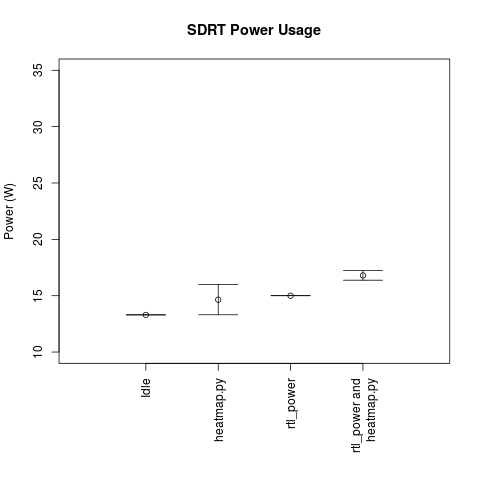
\includegraphics[width=5cm]{images/59}
		\caption{SDRT Power Usage Raspberry Pi B+}
		\label{fig:sdrt_power_usage_pi_b}		
	\end{subfigure}
	\quad
	\begin{subfigure}[t]{5cm}
		\centering
		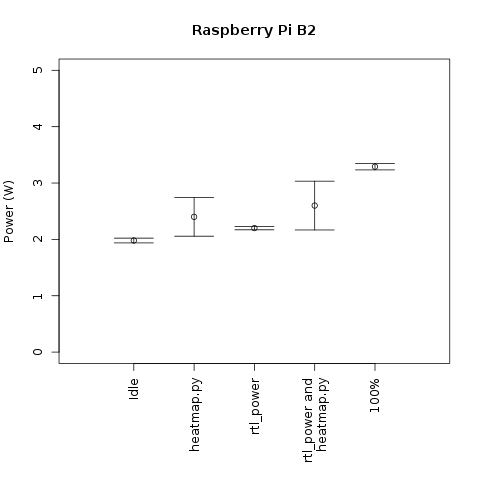
\includegraphics[width=5cm]{images/60}
		\caption{SDRT Power Usage Raspberry Pi B2}
		\label{fig:sdrt_power_usage_pi_b2}
	\end{subfigure}
	\quad
	\begin{subfigure}[t]{5cm}
		\centering
		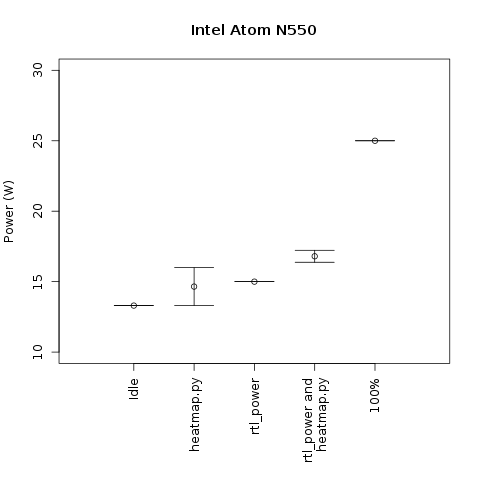
\includegraphics[width=5cm]{images/61}
		\caption{SDRT Power Usage Intel Atom N550}
		\label{fig:sdrt_power_usage_atom_n55}
	\end{subfigure}
	\caption{DAM Emissions}
	\label{fig:jupiter_dam}
\end{figure}
%


\newpage
Using solar data collected by the national weather service, MET Eireann \citep{MET-15} and \citep{ECAD-15}, a period between 1961 and 1977 of solar data was averaged in order to create a series of plots to aid in the calculation of the battery array capacity required to power the system. As can be seen in the Figure.~\ref{fig:barplot_hours_sunshine_waterford} on page~\pageref{fig:barplot_hours_sunshine_waterford}, the mean number of hours of sunlight for this period of time was calculated to be $\mu = 4.446$, with a minimum of 1 hour and a maximum of 9.156 hours.

%
\begin{figure}[here]
	\centering
	\begin{equation}
	Power(Watts) = Current(Ampere) \times Voltage(V)
	\end{equation}
	\begin{equation}
	A = \frac{W}{V}
	\end{equation}
	\begin{equation}
	A = \frac{25}{12}
	\end{equation}
	\begin{equation}
	Ampere = 2.08333333 A
	\end{equation}
	\caption{Calculating Amps using Watts and Voltage}
	\label{fig:power_equation}
\end{figure}
%

Consumer solar panels generally operate at voltages between 12 - 48 V, and should coupled with a battery charge controller, to ensure a battery bank, which may be operating on a lower voltage, can be safely recharged using generated power \citep{bryce-11}. The load power value measured previously for the Intel N550 Netbook operating at 100\% was 25 W. Taking the load and the assumed voltage value of 12 V, the load current was generated using the power equation shown in Equation: \ref{fig:power_equation}. The current required to generate 25 W at 12 V is 2.08333333 A.

An initial estimate of 48 hours of power capacity was made to ensure the system can be powered for an extended period during periods of low solar activity. A plot of load vs battery capacity was generated as shown in Figure.~\ref{fig:lineplot_load_battery_capacity} on page~\pageref{fig:lineplot_load_battery_capacity}. This plot shows the capacity value required to satisfy a 25 W load at 12 V for a 48 hour period is about 100 Ah.

%
\begin{figure}[!htb]
	\centering
	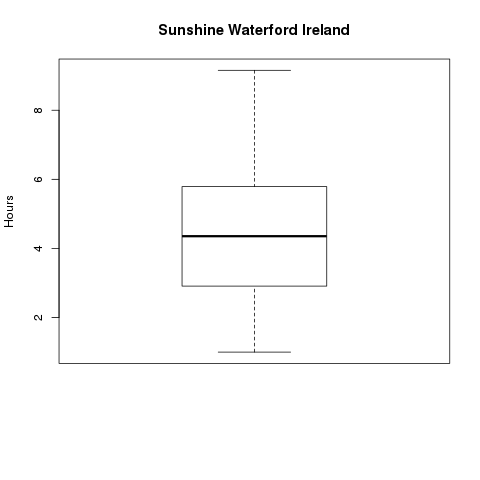
\includegraphics[width=8cm]{images/62}
	\caption{Average Daily Sunshine in Waterford}
	\label{fig:boxplot_hours_sunshine_waterford}
\end{figure}
%

%TODO RQ2 power edit

Figure.~\ref{fig:barplot_hours_sunshine_waterford} on page~\pageref{fig:barplot_hours_sunshine_waterford} shows the averaged daily hours of sunshine over a 15 year period. This plot demonstrates that for half the year the sun shines for between 1 and 4 hours each day. This is a major limiting factor in creating a self sufficient solar powered system, as batteries may only be charged during periods of sunshine. During the times of the year with daily sunshine hours below the mean, a larger battery capacity is required in order to continue to power the system during days with little sunshine. Correspondingly, as the sunshine hours fall, a larger solar panel is required to ensure as much light as possible is converted to energy storage.

%
\begin{figure}	
	\centering
	\begin{subfigure}[t]{5cm}
		\centering
		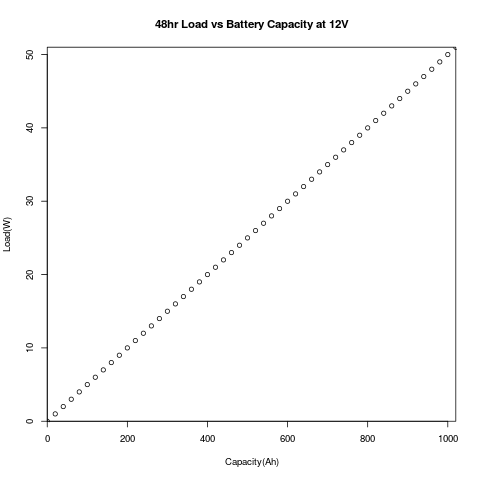
\includegraphics[width=5cm]{images/64}
		\caption{Load vs Battery Capacity Plot}
		\label{fig:lineplot_load_battery_capacity}		
	\end{subfigure}
	\quad
	\begin{subfigure}[t]{5cm}
		\centering
		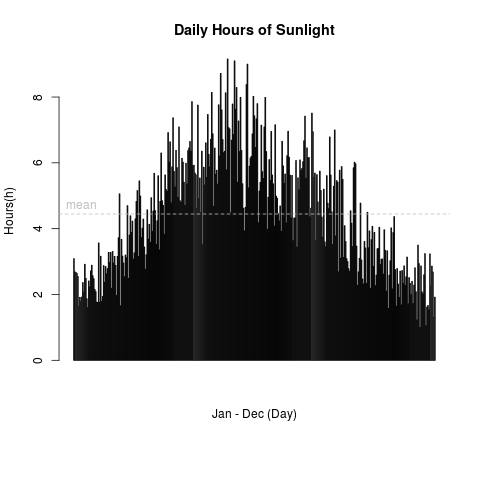
\includegraphics[width=5cm]{images/66}
		\caption{Average Hours of Sunshine per Day in Waterford}
		\label{fig:barplot_hours_sunshine_waterford}
	\end{subfigure}
	\quad
	\begin{subfigure}[t]{5cm}
		\centering
		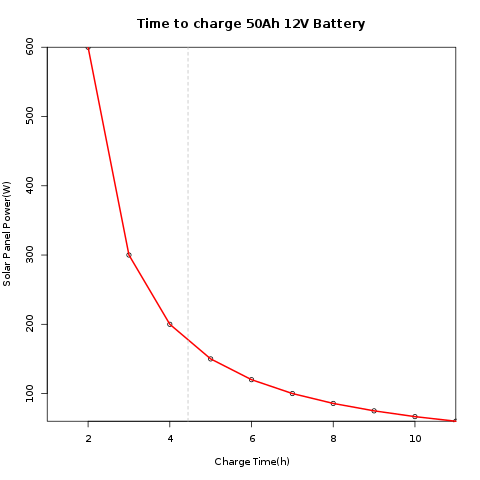
\includegraphics[width=5cm]{images/65}
		\caption{Size of Solar Panel Required to Charge 100Ah Battery in Hours}
		\label{fig:lineplot_solar_panel_battery_capacity_hours}
	\end{subfigure}
	\caption{Solar Plots}
	\label{fig:solar_plots}
\end{figure}
%


Next a plot of solar panel power output vs time taken to charge a 100Ah battery was generated as Figure.~\ref{fig:lineplot_solar_panel_battery_capacity_hours} on page~\pageref{fig:lineplot_solar_panel_battery_capacity_hours}. This plot shows that in order to reliably charge a battery of size 100Ah in a single day which has the mean hours of sunshine the system will require a solar panel array of at least 350W.

The measurements were repeated for the Raspberry Pi systems. The power demands were rounded up to 5W which produced a battery capacity of 20Ah to power for 48 hours. The results were then tabulated as shown in Table: \ref{tab:system_power_requirements}. The components required to implement a solar powered system such as the panels, batteries, charge controller and AC/DC inverters were priced and the results were included in this table also. Price wise, having a Raspberry Pi system in the listening station would make for a cost effective solution. As both the B+ and the B2 versions operate with the very low power usage of 5W, the solar renewable solution would be cheapest also at an estimated \euro 150 for the solar power components.

%
\begin{table}
	\centering
	\begin{tabular}{l r r r}
		\toprule
		Equipment & Solar Panel Power(W) & Battery Capacity(Ah) & Estimated Cost(\euro)\\ \midrule
		Raspberry Pi B+ & 75 & 20 & 150 \\
		Raspberry Pi B2 & 75 & 20 & 150 \\
		Intel Atom N550 & 350 & 100 & 500 \\
		\bottomrule
	\end{tabular}
	\caption{System Power Requirements}
	\label{tab:system_power_requirements}
\end{table}
%


\section*{Determine SDRT Computational Power Requirements}
\addcontentsline{toc}{section}{Determine SDRT Computational Power Requirements}
The aim of this experiment was to determine the minimal hardware which was computationally capable of collecting data, while  performing any data analytical or processing tasks required by the system.


\subsection*{Methodology}
The following platforms were chosen for testing purposes as they initially appear to meet or exceed the minimum requirements of operating rtl\_power while also building spectrograms from the recorded data using heatmap.py:

\begin{enumerate}
	\item Raspberry Pi B+.
	\item Raspberry Pi B 2. 
	\item EEEPC Intel Atom N550 Netbook.
	\item Intel i5-3340M 2.7GHz
\end{enumerate}

Each platform would be measured under a single metric, namely the length of time it takes to produce a spectrogram from data collected over a 24 hour period. Table: \ref{tab:system_cpu_power_requirements} shows the results gathered on each platform. As the time taken to process the spectrogram was longer than 24 hours for both Raspberry Pi models tested, they could not be considered capable of hosting the SDRT system and so this particular test was aborted when the time exceeded 24 hours for both Pi models. 

The Intel Atom powered Netbook performed considerably better with a result of 4.12 hours. This would allow the collection of data, while also the sustainable processing of the previous days data without becoming overloaded.

%
\begin{table}
	\centering
	\begin{tabular}{l r}
		\toprule
		Equipment & Generate Spectrogram(h) \\ \midrule
		Raspberry Pi B+ 800MHz 1 Core & 24Hrs+ \\
		Raspberry Pi B2 900MHz 4 Core & 24Hrs+ \\
		Intel Atom N550 1.55GHz 2 Core & 4.12hours \\
		Intel i5-3340M 2.7GHz 2 Core & 0.25hours \\
		\bottomrule
	\end{tabular}
	\caption{System CPU Power Requirements}
	\label{tab:system_cpu_power_requirements}
\end{table}
%


\newpage
\section*{Determine SDRT Network Connectivity Requirements}
\addcontentsline{toc}{section}{Determine SDRT Network Connectivity Requirements}
The aim of this experiment was to determine the optimal networking technology to transfer collected and or processed data from the SDRT to another system.


\subsection*{Methodology}
The following technologies were investigated during this experiment:

\begin{enumerate}
	\item Zigbee (XBEE Pro 2B 802.15.4)
	\item WIFI (802.11N)
	\item Fast Ethernet (802.3u)
	\item Gigabit Ethernet (802.3-2008)
\end{enumerate}

Each technology was measured using a single metric, transfer speed to copy 2GB of collected data between two nodes in the network. Table: \ref{tab:network_technologies_transfer_time} shows the results obtained. 

%
\begin{table}
	\centering
	\begin{tabular}{p{3cm} l r r }
		\toprule
		Technology & Bitrate & Est(s) & Result(s)\\ \midrule
		Zigbee & 250kbit/s &  76,000 & 24Hrs+ \\
		WIFI N & 144Mbit/s & 132 & 737\\
		Fast Ethernet & 100Mbit/s & 181 & 904 \\
		Gigabit Ethernet & 1Gbit/s & 30 & 45 \\
		\bottomrule
	\end{tabular}
	\caption{Networking technologies transferring 2GB data}
	\label{tab:network_technologies_transfer_time}
\end{table}
%

There existed a large discrepancy between the estimated values and the actual measurements obtained for several technologies measured. A number of factors could account for this, such as the estimated values being generated using theoretical maximum bandwidth for the technology, which are unrealistic for real world applications.

One example is the underlying hardware which handles both the USB and the Fast Ethernet network interfaces on the Raspberry Pi systems has a limit of 2Mbit/s, and could therefore never reach the theoretical maximum of 11Mbit/s suggested by Fast Ethernet. Using the Zigbee XBEE 802.15.4 modules, the theoretical estimate of 250kbit/s suggested a time of 21 hours to transfer 2GB of data, however after 24 hours the transfer was still ongoing. As the ability to the collected data must be faster than the time taken to collect it, the Zigbee test was cancelled after 24 hours. The results show WIFI, and Ethernet technologies being preferable in this instance.
